%!TEX root = handout.tex

\section{Session 3 - Protein Inference}
\label{Session 3 - Protein inference}

\subsection{PIA - Protein Inference Algorithms}
PIA is an open source toolbox for MS based protein inference and identification analysis. It can be used either via a web frontend, KNIME nodes or the command line. While the latter method is intended for advanced scripting, we will introduce the first two methods in this tutorial.

\subsubsection{PIA web frontend}
A demo server for the PIA web frontend is available at \menu{http://134.147.84.213:8080/pia}. Here, you are greeted by a little text and could create a new project from search engine result files. A project in PIA denotes pre-processed search engine results, which can either be derived from single searches or a compilation of results from different search engines or MS/MS runs.

For this tutorial, there are already two projects assembled, which can be accessed from the \menu{Projects} section. To start, open the project \directory{GCB Tutorial} via \menu{Open Project} (do not use the advanced mode right away). This will bring you into the \texttt{wizard-mode}, which will guide you through a default protein inference. The first step is the selection of the score(s) which will be used for the FDR calculation. The \texttt{MS-GF evalue} should be the preferred score for this example, make also sure to uncheck \menu{Create PSM sets} at the top of the page. This option should only be used, when the same MS/MS run was analysed with different search engines. This small example contains only one identification with MS-GF+. The wizard lets you also select the regular expression to identify decoy identifications (which is \texttt{s.*} in this example). Furthermore, you can select whether to use only the best match per spectrum (\menu{only top identification}) or to use all identifications per spectrum. Click on \menu{Calculate FDR} to go to the next page. Here you will get some information calculated on the PSM level as well as a plot of the mass-shift distribution of identified spectra. (If you got a "feeling" for your data, this can be used for a very rough QC.) After clicking on \menu{Show peptides} you will be presented with pie charts, showing how many peptides are identified with how many PSMs.

The next step will bring you to the protein inference. The wizard asks you for the inference method, select the \menu{Spectrum Extractor} for now. If you are interested in how the different methods are working, please look into PIA´s wiki \menu{https://github.com/mpc-bioinformatics/pia/wiki}. The final step is the selection of the used base-score. Select the \menu{PSM FDRScore} and click on \menu{Infere Proteins}. The inference should be finished after some seconds. Afterwards, you are presented with a list of the reported protein groups. If a group has more than one protein, you will see an "Accessions (X)", on which you can click to see every single protein’s accession.

Now switch into the \texttt{advanced mode} to get more details. You will see lots of settings you can play with and the reported list (maybe you have to scroll down to this). This list gives you some more options than the one in the wizard. First, there is a small plus sign (+) to the very left. Clicking on this will show you the peptides of the proteins. The plus always shows you the smaller parts, which constitute the respective row (for peptides PSM sets, for PSM sets finally the PSMs). The small tree-ish icon next to the plus will show you the protein group/peptide/PSM in context, e.g. the reported group with all peptides and PSMs.

\begin{figure}
\centering
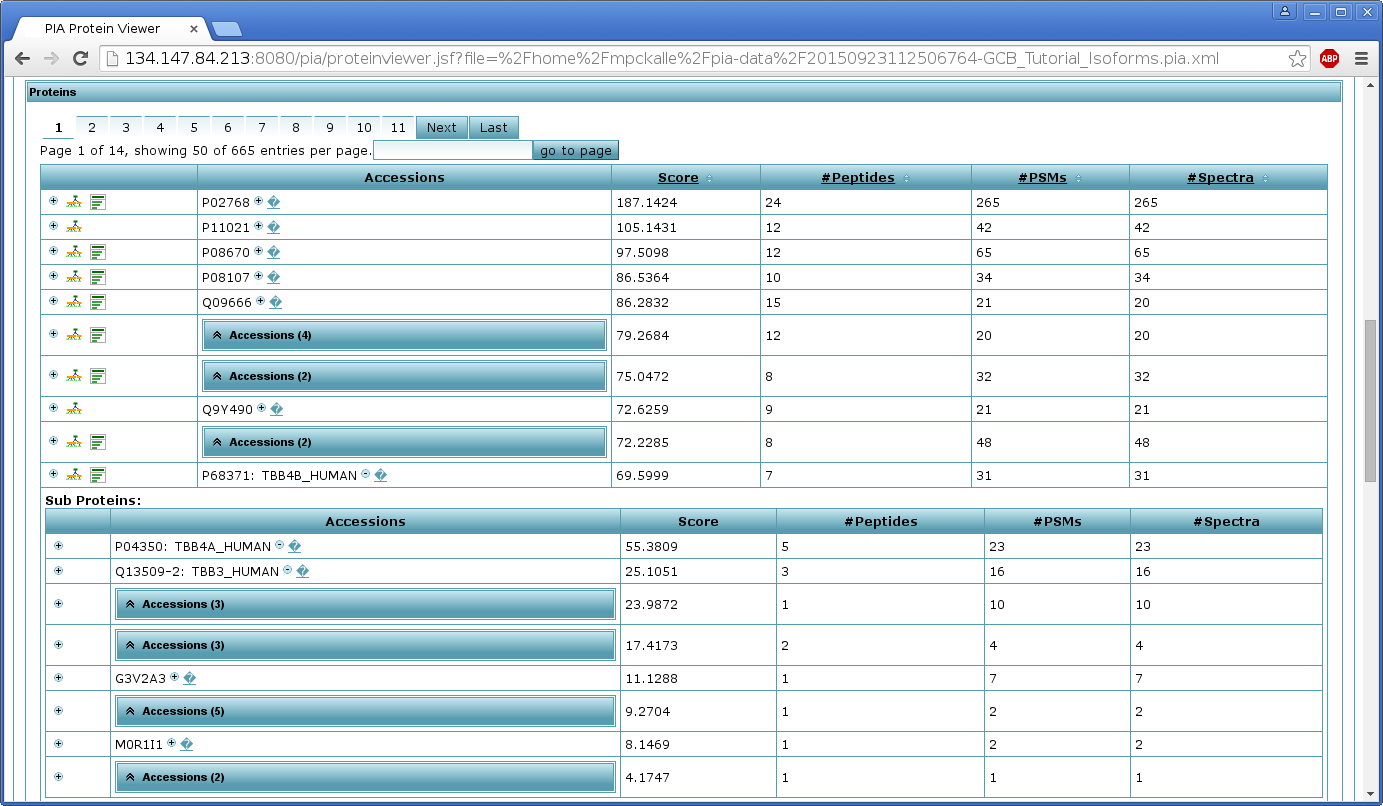
\includegraphics[width=0.7\textwidth]{graphics/protein_inference/pia_protein_list}
\caption{Advanced mode of the PIA protein report in the web frontend.}
\label{fig:pia_advanced_protein}
\end{figure}

\begin{task}
Feel free to explore the web interface, you can filter your results, try another inference or scoring method, or go to the PSM and peptide level. Furthermore (under advanced) you can calculate the FDR and export your reports.
\end{task}


\subsubsection{Installation of PIA KNIME nodes}
To install the PIA KNIME nodes, you need to allow the installation from the nightly (or trunk) repository of KNIME (it will soon be in the stable as well...).

To install PIA go to \menu{Help > Install New Software}. Click on the \menu{available software sites} (directly below the \menu{Add...} button) and then the \menu{Add...} button in the \texttt{Available Software Sites} window. Give the repository a name like \texttt{KNIME trunk} and use the URL \\\menu{http://update.knime.org/community-contributions/trunk}. When everything is entered, click on \menu{OK} and double check, that the just created repository is enabled (checked). Click Ok in the \texttt{Available Software Sites} window and select the trunk repository (or alternatively select \texttt{All available sites}) in the select box. The PIA nodes can be found in the \menu{Bioinformatics \& NGS} group or simply by searching for it. Select it, click next, accept the license and restart KNIME after the installation is finished.

If all went well, you will see the PIA octopus on the splash screen of KNIME and you will find the PIA nodes under \texttt{Community Nodes}. This tutorial also needs the \texttt{OpenMS} and \texttt{R} nodes to be installed, which was explained in the introduction.

The usage of the nodes will be explained in the next section.


\subsection{Protein Inference in KNIME}
Import and open the workflow \directory{GCB\_Tutorial-Protein\_inference.zip} from the USB key into your KNIME workspace. For this tutorial we identify the spectra of the \directory{lfq\_spikein\_dilution\_1.mzML} with MS-GF+ and infere the proteins with PIA and Fido. Below the main workflow is an additional small workflow which will be used later to highlight detection of protein isoforms.
 
\begin{figure}
\centering
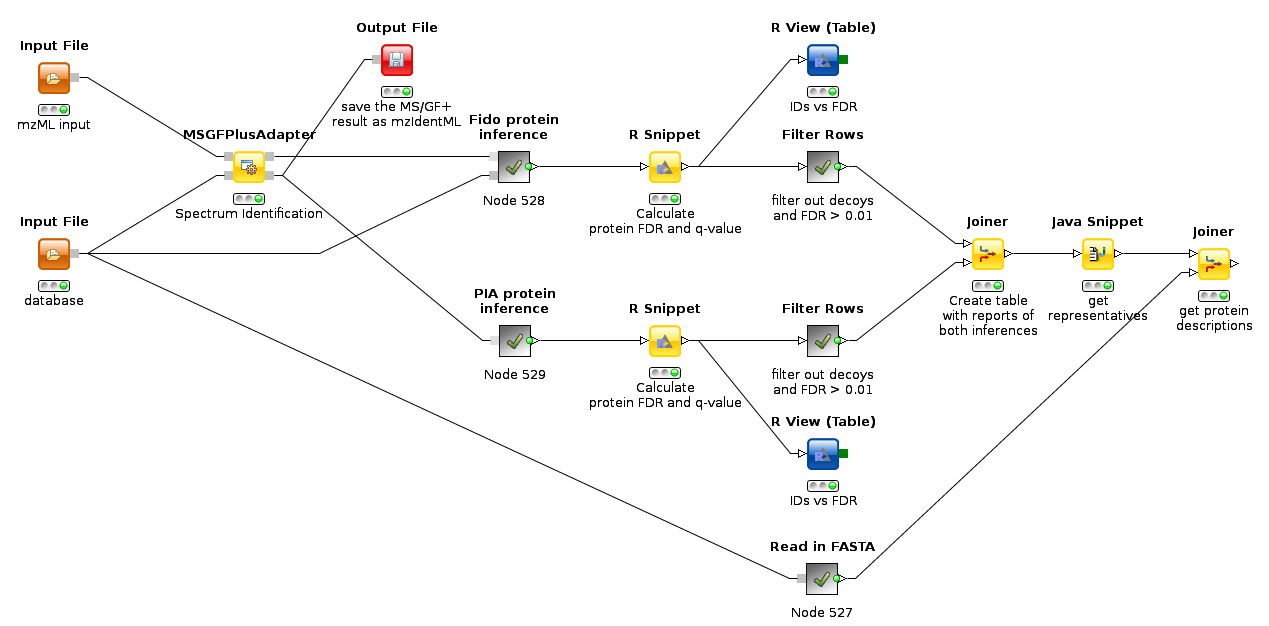
\includegraphics[width=\textwidth]{graphics/protein_inference/inference_workflow}
\caption{A protein inference workflow inferring protein groups with PIA and Fido, as well as creating a simple comparison table.}
\label{fig:pia_and_fido_comparison_workflow}
\end{figure}

To run the workflow, you need to adjust the \KNIMENODE{Input File} nodes, the first one should point to the \directory{lfq\_spikein\_dilution\_1.mzML} and the database input to \newline{}\directory{s\_pyo\_sf370\_potato\_human\_target\_decoy\_with\_contaminants.fasta}, which are both found under \directory{Example\_Data/Labelfree} on the USB key. You need also set the \KNIMENODE{Output File} nodes to valid files on your computer. After setting up all input and output nodes, run the workflow.

The PIA inference can directly use the results of several search engines, including the mzIdentML files created by MS-GF+, but also of all other search engines supported by OpenMS in idXML format. Double click on the \KNIMENODE{PIA protein inference} metanode to further inspect the workflow. As in the web frontend, the result files need to be pre-processed by the \KNIMENODE{PIACompiler} node, which accepts a list of files. The \KNIMENODE{PIAExecute} performs the actual inference, and can also perform all other analyses possible on the web interface. It also exports the data on PSM, peptide and protein level into different formats. Additionally to the compiled identifications, the \KNIMENODE{PIAExecute} needs (at the moment) a pipeline file, which is a bit tricky to generate. The pipeline in the workflow performs roughly the same default workflow as the wizard in the web interface. In the workflow the protein report is saved into an easily parsable CSV format as well as into mzIdentML for later usage in the PRIDE Inspector. The \KNIMENODE{Target decoy classifier} metanode finally reads the data back to KNIME and annotates the decoys.

For the Fido inference it is necessary to calculate posterior probabilities for the PSMs first. Afterwards, the nodes provided by OpenMS to calculate the PSM FDR and filter the results at a 1\% FDR level are used. The filtered PSMs are passed to the \KNIMENODE{FidoAdapter}, which returns the results (like almost all OpenMS nodes) as an idXML file, which makes the metanode necessary to read the data back into KNIME.

After the protein inference, the workflow calculates the protein FDR with R and plots the reported number of target proteins against the FDR q-value. At last, the reported decoys are filtered out and the reports are joined side-by-side into a KNIME table with the protein descriptions.

\begin{task}
    Run the workflow and open the final table to see the differences in the report. You will see, that most of the protein groups are reported by both strategies, PIA and Fido. It is interesting to highlight, that (as explained in the database session) some contaminants are identified, whose accessions start with “CON” in this example. But some groups are also reported by one strategy only. To investigate the reasons for this, either look into the context of these groups in the PIA web frontend, or use PRIDE Inspector for this, which recently integrated parts of PIA and is further explained in the next chapter.
\end{task}


\subsection{PRIDE Inspector}
PRIDE Inspector (PI) is a desktop application to visualise MS data and perform simple quality assessment on Mass Spectrometry data. Recently the ability to perform a simple protein inference and visualisation of this was implemented. The protein inference can be used to briefly inspect files which do not contain protein information, like the results of MS-GF+ searches.

\begin{task}
    To show the protein group visualisation feature, start PI and open the mzIdentML file generated by PIA \directory{lfq\_spikein\_dilution\_1-pia.mzId}. If you did not create the filed on your own, they are also located under \directory{Example\_data/session3-protein\_inference}. It is up to you to also load the spectra data from the corresponding mzML file. In KNIME we saw, that several groups were reported by Fido, but not PIA. Let’s search for the protein group containing J7MBF9 and Q99XR9, which was reported by both inferences. Go to the \menu{Proteins} tab and click \menu{Ctrl > F} and enter one of the accessions.
    
    Click on "show protein groups" and you will see something similar to the visualization in PIA’s web frontend. You can uncollapse the proteins and will see that J7M5J8 and Q9A086 is a sub-group of J7MBF9 and Q99XR9 and is therefore not reported by PIA. Fido assumes enough significance for the sub-group and reports it, though. You will find similar reasons for the other, differently reported protein groups.
\end{task}

\begin{figure}
\centering
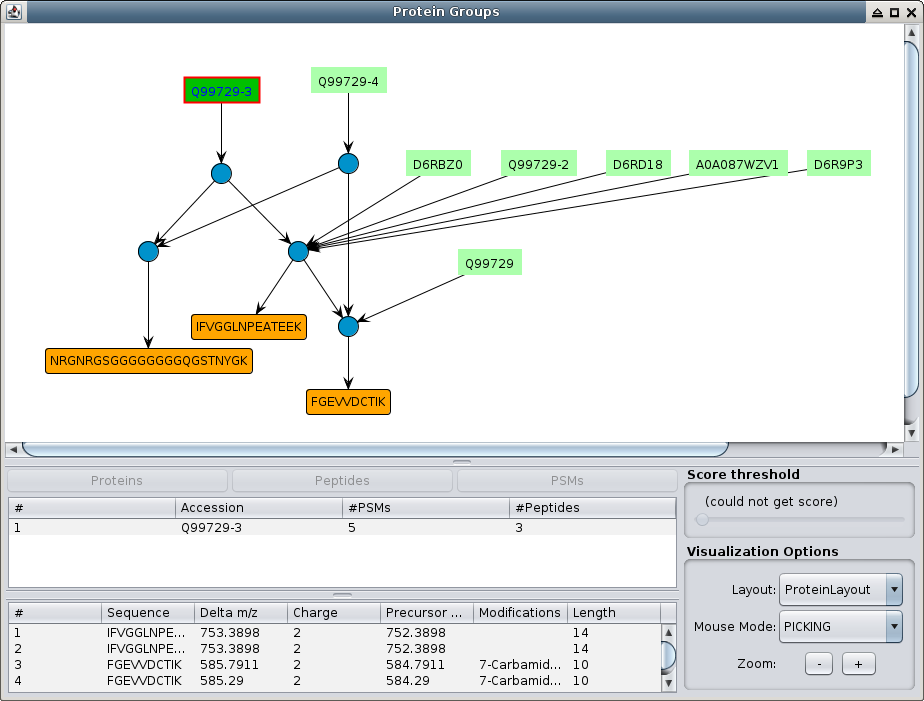
\includegraphics[width=0.7\textwidth]{graphics/protein_inference/inference_isoforms}
\caption{Visualisation of protein groups in the PRIDE Inspector. If an accession is selected, the peptides which are connected to the accession are in dark orange, accessions with the same peptides (i.e. in the same group) are dark green. Protein groups which contain all the peptides of the selected accession but also some additional peptides are light green with a dark green border. This makes it easy to see the context of proteins, peptides and PSMs. The blue nodes are only necessary to maintain the structural overview.}
\label{fig:pride_inspector_protein_groups}
\end{figure}


\subsection{Detection of Isoforms}
If the data was searched with a database containing isoforms, it can be interesting to see, whether there was any evidence that one of the isoforms was detected. For this, there was a small sub-workflow in the main workflow which uses as database the Human Complete Proteome of Uniprot with isoforms and makes a protein inference with PIA. The resulting file is saved in LC2-pia.mzId. (LC stands for lung cancer in this example).

\begin{task}
    You can either use the PRIDE Inspector or the PIA web frontend with the \directory{GCB Tutorial Isoforms} to investigate some isoforms, e.g. Q99729-3 which has a unique peptide to distinguish it from the other isoforms of Q99729.
\end{task}
